\section{Закон Био-Савара-Лапласа}

%1
\AddProb Ток $I$ течет по длинному прямому проводнику, сечение которого имеет форму тонкого полукольца радиуса $R$. Найти магнитную индукцию на оси~$O$.

\begin{wrapfigure}{r}{2.5cm}
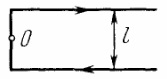
\includegraphics[scale=0.4]{1202BiotSavartLawConductor.jpg}
\end{wrapfigure}

\AddProb Найти модуль и направление силы, действующей на единицу длины тонкого проводника с током $I$ в точке $O$, 
если проводник изогнут так, как показано на рисунке.


\section{Сила Ампера}

\begin{wrapfigure}{r}{4cm}
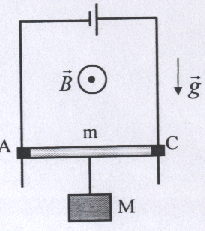
\includegraphics[width = 4cm]{RodInMagneticField.png}
\end{wrapfigure}
\AddProb (2016) На рисунке представлена модель электродвигателя. Замкнутый контур образован двумя вертикальными рейками, между концами которых включен источник постоянного тока с ЭДС {\Large $\varepsilon$}, a другие концы замкнуты перемычкой сопротивлением $R$ и длиной $L$. Перемычка за счет скользящих контактов может без трения скользить вдоль реек. Контур находится в однородном магнитном поле с индукцией $B$, направленной горизонтально. Известно, что если к перемычке подвесить груз массы $M$, она будет в состоянии равновесия. 1) Определите массу $m$ перемычки. 2) Определите установившуюся скорость ненагруженной перемычки. Сопротивлением реек и внутренним сопротивлением источника пренебречь.

\AddProb (2003) Металлический стержень массой $m$ и длиной $L$ подвешен на двух легких проводах длиной $l$ в магнитном поле с индукцией $B$, 
вектор которой направлен вертикально. К точкам крепления проводов подключен конденсатор емкостью $C$, заряженный до напряжения $U$. 
Сопротивление стержня и проводов пренебрежимо мало. Найти максимальный угол отклонения проводов от вертикали, 
если разрядка конденсатора происходит за очень малое время.

\begin{wrapfigure}{r}{4.5cm}
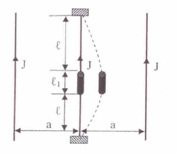
\includegraphics[scale=1]{122010AmperesForceLawTwoConductors.jpg}
\end{wrapfigure}

\AddProb (2010) Посередине между двумя жестко закрепленными проводниками с током на расстоянии $a$ расположен груз массы $m$, 
представляющий собой цилиндрическую железную трубку длиной $l_1$ и укрепленный с помощью упругих растяжек длиной $l$. 
Магнитная проницаемость железа $\mu$. Внутри растяжек установлен еще один проводник. По всем трем проводникам течет ток $J$. 
Определите собственную частоту свободных колебаний груза, считая, что в процессе колебаний натяжение растяжек $T_0$ не изменяется. 
Определить зависимость критического значения силы тока от натяжения растяжек, считая критическим значением такое значение, 
при котором колебания в системе невозможны.

\begin{wrapfigure}{r}{3cm}
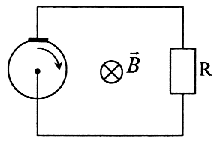
\includegraphics[width = 3cm]{AmperGenerator.png}
\end{wrapfigure}
\AddProb (2017) Одна из моделей генератора постоянного тока представляет собой проводящий диск, который вращается в однородном магнитном поле с индукцией,
направленной перпендикулярно плоскости вращения диска. Если концы некоторого проводника сопротивлением $R$ присоединить к центру диска и через скользящий контакт к его ободу, то в цепи возникнет электрический ток. 1) Объясните
возникновение электрического тока и найдите силу тока, если радиус диска $r = 10$ см, частота вращения диска $\nu = 40$ об/с, индукция магнитного поля $B = 0,1$ Тл, сопротивление нагрузки $R = 0,5$ Ом. 2) Какая мощность затрачивается для поддержания вращения диска? 3) Какой момент силы относительно оси вращения нужно прикладывать к диску? Сопротивлениями диска и контактов пренебречь.


\section{Теорема о циркуляции индукции магнитного поля}

\begin{wrapfigure}{r}{3cm}
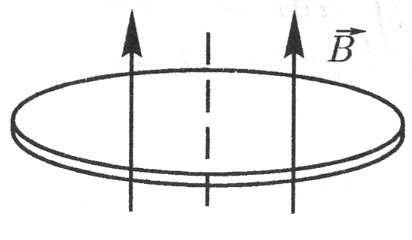
\includegraphics[scale=0.25]{1205AmperesCircuitalLawDisc.jpg}
\end{wrapfigure}

\AddProb Однородный диэлектрический диск массой $m$ радиуса $R$, равномерно заряженный с полным зарядом $q$, 
помещен в однородное магнитное поле с индукцией $B$. Какую угловую скорость получит диск, если выключить магнитное поле?

\begin{wrapfigure}{r}{4cm}
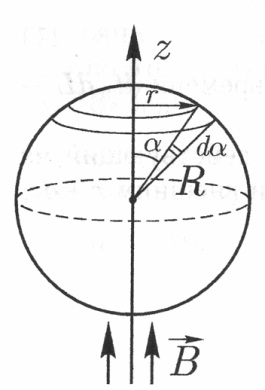
\includegraphics[scale=0.5]{1206AmperesCircuitalLawSphere.jpg}
\end{wrapfigure}

%6
\AddProb По поверхности жесткой непроводящей однородной сферы массой $m$ равномерно распределен заряд $q$. 
Сфера может свободно вращаться вокруг своей вертикальной оси. В начальный момент сфера покоилась, а магнитное поле было равно нулю. 
Найти, как меняется со временем угловая скорость сферы при включении однородного магнитного поля, 
сонаправленного с осью вращения сферы и меняющегося во времени по заданному закону $B(t)$.


\section{Электромагнитная индукция}

\begin{wrapfigure}{r}{4cm}
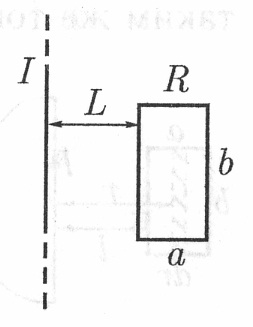
\includegraphics[scale=0.5]{122002EMIFrame.jpg}
\end{wrapfigure}

\AddProb (2002) Прямоугольная рамка со сторонами $a$ и $b$ находится в одной плоскости с прямым проводником, 
по которому течет ток $I$, на расстоянии $L$ от него. Какой импульс получит рамка при выключении тока в проводе, 
если активное сопротивление рамки равно $R$, а реактивным сопротивлением ее можно пренебречь? 
Считать, что за время передачи импульса рамка заметно не перемещается.

\AddProb (2001) На расстоянии $a$ и $b$ от длинного прямого провода с током $I$ расположены два параллельных ему провода, 
замкнутые с одной стороны сопротивлением $R$. По проводам без трения перемещаются с постоянной скоростью $v$ стержень-перемычку. 
Пренебрегая сопротивлением проводов, стержня и контактов, найдите силу, необходимую для поддержания постоянства скорости. 
На каком расстоянии от ближнего провода нужно приложить силу, чтобы избежать вращения стержня?

\begin{figure}[!h]
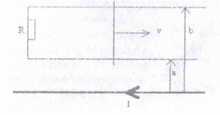
\includegraphics[scale=0.9]{122001EMIWiresAndBar.jpg}
\end{figure}

\AddProb (2004) Металлический стержень массы $m$ и длины $L$ подвешен горизонтально на двух легких проводах длиной $h$ в магнитном поле, 
индукция которого $B$ направлена вертикально вниз. К точкам крепления проводов подключен конденсатор емкостью $C$. 
Стержень вывели из положения равновесия и отпустили. Определить период малых колебаний стержня $T$. Сопротивлением стержня и проводов пренебречь.

\begin{wrapfigure}{r}{2cm}
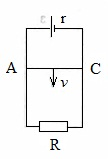
\includegraphics[scale=0.5]{121998EMIConductorAC.jpg}
\end{wrapfigure}

\AddProb (1998) По двум вертикальным рейкам, соединенным внизу сопротивлением $R$ и вверху источником с ЭДС {\Large $\varepsilon$} 
и внутренним сопротивлением $r$, без трения скользит проводник $AC$, длина которого $L$, масса $m$. 
Система находится в однородном магнитном поле с индукцией $B$, направленной за рисунок. 
Найдите установившуюся скорость проводника в поле силы тяжести, пренебрегая трением и сопротивлением реек и проводника.

\begin{wrapfigure}{r}{4cm}
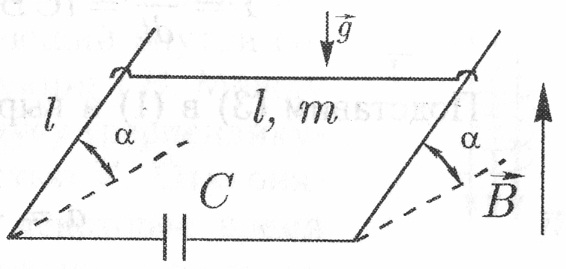
\includegraphics[scale=0.25]{1211EMIHillAndBridge.jpg}
\end{wrapfigure}

%11
\AddProb По двум параллельным металлическим направляющим, наклоненным под углом $\alpha$ к горизонту и 
расположенным на расстоянии $l$ друг от друга, может скользить без трения металлическая перемычка массой $m$. 
Направляющие замкнуты снизу на незаряженный конденсатор емкостью $C$, и вся конструкция находится в магнитном поле, 
индукция которого $B$ направлена по вертикали. В начальный момент перемычку удерживают на расстоянии $l$ от основания "горки". 
Определите время $t$, за которое перемычка достигнет основания "горки" после того, как ее отпустят. 
Омическим сопротивлением и индуктивностью контура пренебречь.

\AddProb (2001) Две параллельные медные шины наклонены к горизонту под углом  $\alpha$. 
По ним скользит под действием силы тяжести медная перемычка массы $m$. Шины замкнуты катушкой с индуктивностью $L$. 
Система находится в однородном магнитном поле индукции $B$, перпендикулярном плоскости, в которой движется перемычка. 
Коэффициент трения перемычки о шины равен $\mu$. Каков будет характер движения перемычки? Сопротивлением шин, перемычки и катушки пренебречь.

\begin{wrapfigure}{r}{4.5cm}
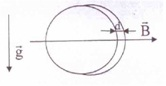
\includegraphics[scale=1]{122009EMICoin.jpg}
\end{wrapfigure}

\AddProb (2009) Медная монета массой $m$ радиусом $R$ и толщиной $d$ движется в поле силы тяжести в однородном магнитном поле $B$. 
Вектор индукции магнитного поля направлен вдоль оси монеты и перпендикулярно ускорению свободного падения. Найти ускорение монеты.

\begin{wrapfigure}{r}{5cm}
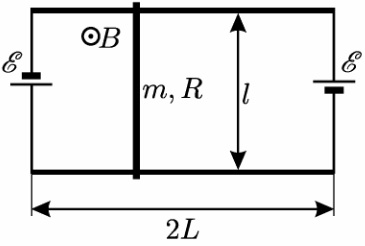
\includegraphics[scale=0.5]{1214EMIRailsAndBridge.jpg}
\end{wrapfigure}

\AddProb Параллельные рельсы длиной $2L$ закреплены на горизонтальной плоскости на расстоянии $l$ друг от друга. 
К их концам подсоединены две одинаковые батареи с ЭДС {\Large $\varepsilon$}. На рельсах лежит перемычка массы $m$, 
которая может поступательно скользить вдоль них. Вся система помещена в однородное вертикальное магнитное поле с индукцией $B$. 
Считая, что сопротивление перемычки равно $R$, а сопротивление единицы длины каждого из рельсов равно $\rho$, найдите период малых колебаний, 
возникающих при смещении перемычки от положения равновесия, пренебрегая затуханием, внутренним сопротивлением источников, 
сопротивлением контактов, а также индуктивностью цепи.

\AddProb (2015) Проводящая квадратная рамка пересекает область однородного магнитного поля с шириной $d$, линии напряженности которого перпендикулярны плоскости рамки. При этом скорость рамки, равная $v_0$ до входа в магнитное поле уменьшается в 2 раза Масса рамки равна $m$, сопротивление рамки — $R$, величина вектора магнитной индукции - $B$. 1) Объясните, почему в рамке при пересечении магнитного поля выделяется тепло и найдите его. 2) Определите длину стороны рамки $a$ предполагая, что $a<d$. 3) Определите длину стороны рамки $a$ предполагая, что $a>d$.

\section{Движение заряженных частиц}

\AddProb Заряженная частица массы $m$ влетает в магнитное поле $B$ под углом $\alpha$ со скоростью $v$. По какой траектории движется частица? Каков пространственный период витка (шаг спирали)?

%Зональные студенческие олимпиады Ижевска
\AddProb По обмотке длинного цилиндрического соленоида радиуса R протекает постоянный ток, создающий внутри соленоида однородное магнитное поле с индукцией $B$. Между витками соленоида в него влетает по радиусу (перпендикулярно оси соленоида) электрон со скоростью $v$. Отклоняясь в магнитном поле, электрон спустя некоторое время покинул соленоид. Определите время движения внутри соленоида.

\AddProb (2008) Электронно-лучевая трубка помещена в однородное магнитное поле, напряженность $H$ которого перпендикулярна плоскости экрана. Электроны влетают в электронно-лучевую трубку из электронной пушки с составляющей скорости $u$ вдоль оси трубки и составляющей скорости $v_0$ перпендикулярно оси. При какой длине $L$ трубки все электроны фокусируются в одной точке экрана?

\AddProb (2012) Две заряженные частицы движутся в однородном магнитном поле $B$, причем $q_1/m_1 = q_2/m_2$. Написать уравнения движения центра масс и уравнение относительного движения.

%16
\AddProb (2013) Заряд $q$ движется в поле магнитного монополя $\vec{B} = \alpha \vec{r}/r^3$. Найдите интеграл движения, следующий из закона изменения момента импульса заряда.

\AddProb Частица c зарядом $q$ и массой $m$ движется с начальной скоростью $v_0$ в вязкой среде в поперечном магнитном поле с индукцией $B$. Сила сопротивления $\vec{F} = -\gamma \vec{v}$, где $\gamma$ - константа. На каком расстоянии от начальной точки частица остановится?

\AddProb (2007) Частица c зарядом $q$ и массой $m$ движется в постоянных однородных скрещенных полях $\vec{E} \bot \vec{H}$ в среде с малым линейным сопротивлением $\vec{F} = -\gamma \vec{v}$. Найти скорость частицы вдоль поля $\vec{E}$, усредненную по периоду.

%Зональные студенческие олимпиады Ижевска, Черепанов
\AddProb На магнитный барьер, задаваемый в пространстве статическим магнитным полем $\vec{B} = \left(0, 0, \frac{B_0}{\cosh^2(ky)}\right)$, где $k$ - константа, из бесконечности налетает протон с начальной скоростью $\vec{v}_{-\infty} = (0, v_0, 0)$, $\vec{r}_{-\infty} = (0, -\infty, 0)$. Оцените минимальную скорость, которую должен иметь протон, чтобы преодолеть барьер и уйти на бесконечность. 

\begin{wrapfigure}{r}{5cm}
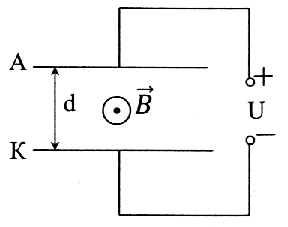
\includegraphics[scale=0.6]{ElectronInVacuumDiode.png}
\end{wrapfigure}
\AddProb (2018) Вакуумный диод представляет собой две металлические пластины -- катод и анод. Между пластинами имеется однородное магнитное поле с индукцией $B$, параллельной плоскости пластин (направленной из плоскости чертежа). Расстояние между пластинами $d$. Из катода вылетают электроны. 1) При каких начальных скоростях все электроны не смогут достичь анода при $U = 0$? 2) При каких напряжениях $U$ все электроны не смогут достичь анода при нулевой начальной скорости?

\section{Колебательный контур}

\begin{wrapfigure}{r}{3.5cm}
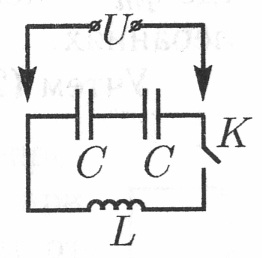
\includegraphics[scale=0.5]{1219OscillatoryCircuitCCL.jpg}
\end{wrapfigure}

\AddProb Батарея из двух последовательных соединенных конденсаторов емкостью $C$ каждый заряжена до напряжения $U$ 
и в начальный момент времени подключена к катушке индуктивностью $L$, так что образовался колебательный контур. 
Спустя интервал времени $\tau$ один из конденсаторов пробивается, и сопротивление между обкладками становится равным нулю. 
Найдите амплитуду колебаний заряда на непробитом конденсаторе.

\begin{wrapfigure}{r}{4cm}
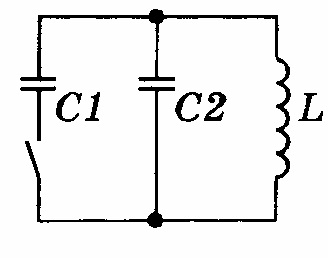
\includegraphics[scale=0.4]{1220OscillatoryCircuitC1C2L.jpg}
\end{wrapfigure}

\AddProb Два конденсатора одинаковой электроемкости $C_1~=~C_2~=~C$ и катушка индуктивности $L$ соединены так, как показано на рисунке. 
В начальный момент времени ключ разомкнут, конденсатор $C_1$ заряжен до разности потенциалов $U$, а конденсатор $C_2$ не заряжен, 
сила тока в катушке равна нулю. Определите максимальное значение силы тока в катушке после замыкания цепи и период электромагнитных колебаний в цепи. 

\begin{wrapfigure}{r}{3.5cm}
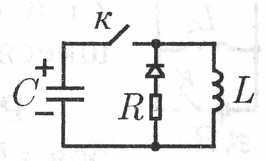
\includegraphics[scale=0.5]{1221OscillatoryCircuitCLR.jpg}
\end{wrapfigure}

%21
\AddProb В схеме, изображенной на рисунке, в некоторый момент времени замыкают ключ $K$, и конденсатор емкостью $C$, 
имеющий первоначальный заряд $q_0$, начинает заряжаться через катушку индуктивности $L$. 
Когда ток разряда достигает максимального значения, ключ $K$ вновь размыкают. Найти заряд $Q$, который протечет через резистор $R$. 
Сопротивление диода в прямом направлении много меньше $R$, в обратном - бесконечно велико.

\begin{wrapfigure}{r}{3.5cm}
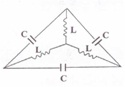
\includegraphics[scale=1]{122011OscillatoryCircuitTriangleCCCLLL.jpg}
\end{wrapfigure}

\AddProb (2011) Электрический контур представляет собой треугольник, каждая сторона которого содержит емкость $C$, 
а вершины соединены с общей центральной точкой индуктивностями $L$. 
Пренебрегая сопротивлением и взаимной индуктивностью, найдите частоту возможных колебаний.


\section{Переменный электрический ток}

\begin{wrapfigure}{r}{2cm}
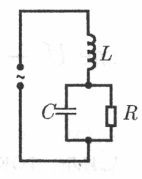
\includegraphics[scale=0.4]{1223AlternatingCurrentCLR.jpg}
\end{wrapfigure}

\AddProb В изображенной на рисунке электрической цепи определите частоту приложенного переменного напряжения, 
при которой переменный ток через сопротивление не зависит от значения $R$. Индуктивность $L$ и емкость $C$ считать известными.

\AddProb При каком условии амплитуда тока в цепи зависит только от амплитуды приложенного напряжения, 
но не от его частоты? Индуктивность $L$, и емкость $C$, и сопротивление $R$ считать известными.

\begin{figure}[!h]
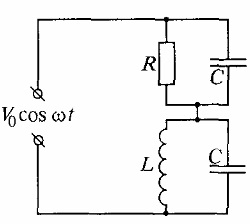
\includegraphics[scale=0.5]{1224AlternatingCurrentCCLR.jpg}
\end{figure}

\AddProb В приведенной на рисунке схеме в момент $t$~ =~0 замыкают ключ $K$. Найти зависимость от времени тока $I$, 
текущего через источник синусоидальной ЭДС {\Large $\varepsilon$}~=~{\Large $\varepsilon_o$}\,$\sin\,\omega\,t$.
%$\varepsilon\,=\,\varepsilon_0\,\sin\,\omega\,t$.  
Параметры контура связаны соотношением $R\,=\,\sqrt{L/C}$.

\begin{figure}[!h]
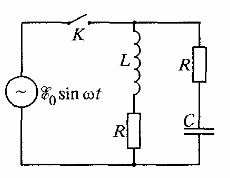
\includegraphics[scale=0.5]{1225AlternatingCurrentCLRR.jpg}
\end{figure}